\documentclass[conference]{IEEEtran}
\usepackage{graphicx,booktabs,amsmath,amssymb,url,xcolor,tikz,algorithm,algpseudocode,multirow}
\usetikzlibrary{arrows.meta,positioning,fit}
\usepackage[hidelinks]{hyperref}
\graphicspath{{../results/figures/}{figures/}}
\newcommand{\tbl}[1]{\IfFileExists{tables/#1}{\input{tables/#1}}{\multicolumn{3}{l}{(pending: #1)}\\}}
\newcommand{\fig}[2]{\IfFileExists{../results/figures/#1}{\includegraphics[width=#2]{#1}}{\IfFileExists{figures/#1}{\includegraphics[width=#2]{#1}}{\fbox{\parbox{0.9\columnwidth}{\centering pending: #1}}}}}

\begin{document}
\title{Evidence-Grounded Clinical-Trial Criterion Matching with a LoRA-Adapted Small Transformer, KV-Cached, Tiled-Attention and Speculative Inference}

\author{\IEEEauthorblockN{Abdullah Tahir (i210708)}
\IEEEauthorblockA{Generative AI --- Assignment 2\\ GitHub: \url{https://github.com/Abdullah8168/trialgpt-criterion-matching}}}
\maketitle

\begin{abstract}
We build and evaluate a complete, locally executable system that judges whether a patient
description satisfies an individual inclusion or exclusion criterion of a clinical trial and
grounds every judgement in numbered sentences of the patient record. Qwen2.5-1.5B-Instruct is
adapted with Low-Rank Adaptation (LoRA) on the TrialGPT Criterion Annotations dataset under a
fixed patient-grouped 37/8/8 split. It outputs a structured JSON object with one of the four
expert label categories (including \emph{not enough information} and \emph{not applicable})
and supporting sentence IDs. We compare the same model before and after fine-tuning on
identical held-out examples, and report label and evidence metrics overall and separately for
inclusion and exclusion criteria. We also implement the inference stack from first
principles: an explicit key/value-cached decoder validated token-for-token against an
uncached reference, a tiled online-softmax attention kernel validated against reference
scaled dot-product attention, and greedy speculative decoding with a fine-tuned 0.5B draft
model and explicit cache rollback. All components are exposed in a browser application that
produces downloadable, provenance-stamped screening reports. On the held-out test patients, fine-tuning
raises accuracy from 0.170 to 0.704, macro-F1 from 0.158 to 0.434 and evidence micro-F1 from 0.183 to 0.545.
The adapted model nevertheless collapses towards majority labels for exclusion criteria. The cached decoder is
token-identical to the reference and 2--7$\times$ faster. The tiled kernel matches reference attention to fp16
precision with linear instead of quadratic memory. Speculative decoding is exact but 6--26\% slower on a T4,
and we explain why.
\end{abstract}
\begin{IEEEkeywords}
clinical trial matching, large language models, LoRA, KV cache, online softmax, FlashAttention, speculative decoding
\end{IEEEkeywords}

\section{Introduction}
Recruitment is a major bottleneck of clinical research. Screening a patient means checking
dozens of free-text criteria against an unstructured clinical note. TrialGPT~\cite{jin2024trialgpt}
showed that large language models (LLMs) can perform criterion-level matching with
explanations, but it relies on a proprietary API model (GPT-4). This work asks whether a
\emph{small, open-weight, locally executable} Transformer can be adapted to the same
criterion-level task under strict data hygiene, while making every decision traceable to
evidence sentences.

\textbf{Problem statement.} Given (i) a patient note split into sentences $s_0,\dots,s_{n-1}$,
(ii) a criterion type $t\in\{\text{inclusion},\text{exclusion}\}$ and (iii) a criterion text $c$,
predict a label $y\in\mathcal{Y}_t$ and an evidence set $E\subseteq\{0,\dots,n-1\}$. Here
$\mathcal{Y}_{\text{inc}}=\{$included, not included, not enough information, not applicable$\}$ and
$\mathcal{Y}_{\text{exc}}=\{$excluded, not excluded, not enough information, not applicable$\}$.
The categories are never collapsed to yes/no, and absence of evidence is never treated as proof.

\textbf{Contributions.} (1) A reproducible LoRA fine-tuning and evaluation pipeline on the
prescribed split, with before/after comparison. (2) Hand-written KV-cached, tiled-attention
and speculative decoders with correctness tests and synchronized benchmarks. (3) A browser
screening application with rule-based aggregation, missing-information reporting and report
export. (4) An error analysis of the failure modes.

\section{Related Work}
\textbf{Patient--trial matching.} TrialGPT~\cite{jin2024trialgpt} decomposes matching into
criterion-level prediction (TrialGPT-Matching), trial-level ranking and retrieval. Its
criterion annotations, built on the SIGIR 2016 patient collection~\cite{koopman2016test}, are the
benchmark used here. TrialGPT uses GPT-4 zero-shot. We instead adapt a model 100$\times$ smaller
with supervision, trading general reasoning for locality, privacy and cost.

\textbf{Architectures.} Decoder-only Transformers~\cite{vaswani2017attention} with rotary position
embeddings (RoPE)~\cite{su2024roformer} and grouped-query attention (GQA)~\cite{ainslie2023gqa}
dominate open-weight LLMs. The Qwen2.5 family~\cite{qwen2025} and Llama~3.2~\cite{grattafiori2024llama}
offer 0.5--3B models that fit free GPUs.

\textbf{Parameter-efficient adaptation.} LoRA~\cite{hu2022lora} freezes pretrained weights and learns
low-rank updates $\Delta W=BA$, cutting trainable parameters by about 100$\times$. QLoRA~\cite{dettmers2023qlora}
adds 4-bit quantization of the frozen base. Full fine-tuning of a 1.5B model needs about 24\,GB of optimizer
state and does not fit a 16\,GB T4.

\textbf{Efficient inference.} KV caching turns per-step decoding cost from $O(t)$ re-encoding into
$O(1)$ new-token work~\cite{pope2023efficiently}. PagedAttention~\cite{kwon2023vllm} manages cache memory at
serving scale. Online softmax~\cite{milakov2018online} enables FlashAttention~\cite{dao2022flashattention},
which tiles attention to avoid materializing the $L\times L$ score matrix. Speculative
decoding~\cite{leviathan2023fast,chen2023accelerating} uses a cheap draft model and verifies its proposals in one
target pass, so the output is identical to the target's under greedy acceptance.

\textbf{Limitations of prior work for our setting.} API-based GPT-4 cannot be run locally or
inspected. FlashAttention's CUDA kernels need specific GPUs. Library assisted generation hides the
cache logic the assignment asks us to implement and explain. These gaps motivate our design.

\section{Materials and Methods}
\subsection{Dataset and Fixed Split}
The TrialGPT Criterion Annotations dataset~\cite{jin2024trialgpt} has 1,015 criterion-level
annotations covering 53 patients and 103 trials. Each record includes a numbered patient note,
the criterion type and text, the expert label and the expert evidence-sentence IDs. The
columns \texttt{gpt4\_explanation}, \texttt{gpt4\_sentences}, \texttt{gpt4\_eligibility} and
\texttt{explanation\_correctness} hold previous model outputs and are \emph{dropped at load
time} (asserted in code). The dataset's own \texttt{training} flag is ignored. One record with a null
criterion text is removed. Unique patient IDs are sorted, shuffled with
\texttt{numpy.random.default\_rng(42)} and assigned 37/8/8 to train/validation/test. A leakage check
asserts that every patient belongs to exactly one split and that pairwise intersections are empty.
Table~\ref{tab:split} summarizes the split. The full manifest (patient IDs, label counts) is
published as \texttt{data/split\_manifest.json}. The data are highly imbalanced: \emph{not excluded}
and \emph{not enough information} dominate, and the test split has no \emph{excluded} example. Inclusion
and exclusion macro-F1 are therefore computed over the classes present in the gold labels.

\begin{table}[t]\centering\caption{Patient-grouped split (seed 42).}\label{tab:split}
\begin{tabular}{lrrrrr}\toprule
Split & Pat. & Ann. & Incl. & Excl. & w/ gold evid.\\\midrule
\tbl{split.tex}
\bottomrule\end{tabular}\end{table}

\subsection{Input/Output Format and Tokenization}
Each example becomes a chat prompt (Qwen chat template) with a system instruction, the note
rendered as ``\texttt{i. sentence}'' lines with the dataset's original sentence IDs, the
criterion type, the criterion text and the allowed labels for that type. The target is the
compact JSON \texttt{\{"evidence": [3, 4], "label": "included"\}} followed by
\texttt{<|im\_end|>}. Evidence comes \emph{before} the label so that the label is decoded
conditioned on the cited sentences. Tokenization uses Qwen2.5's byte-level BPE (151k vocabulary).
\textbf{Truncation.} The prompt budget is 1,024 tokens. When it is exceeded, trailing note sentences are
dropped and the event is logged, together with whether gold evidence was lost. Measured prompts
average 338 tokens (p95 481, max 623), so \emph{no record was truncated} and no evidence was lost.

\textbf{Explanations.} The dataset contains no expert explanations, and the GPT-4 explanations
must not be used. The system therefore composes each explanation deterministically from the label and
the verbatim cited sentences, and flags weakly supported decisive labels that cite no sentence. Every
explanation can thus be traced to the source record.

\subsection{Model Selection}
Table~\ref{tab:models} compares the candidates. Hardware was a free Kaggle NVIDIA T4 (16\,GB, no bf16)
for training and a local GTX~1650 (4\,GB) for the application. \textbf{Qwen2.5-1.5B-Instruct} was chosen
for these reasons. It has an Apache-2.0 license and ungated weights. Its 3.1\,GB fp16 footprint fits
the 4\,GB local GPU for inference, and fp32 frozen weights (6.2\,GB) plus LoRA fit the T4 for training.
GQA with only 2 KV heads gives a cache of just 28\,KB/token ($2\times28$ layers $\times2$ heads
$\times128$ dims $\times2$ bytes). Most importantly, it has a same-tokenizer 0.5B sibling to serve as
the speculative draft. Llama-3.2-1B was rejected because its license is gated and its smallest
compatible draft is not smaller by a useful margin. Phi-3.5-mini (3.8B) does not fit 4\,GB at fp16.

\begin{table}[t]\centering\caption{Open-weight decoder candidates.}\label{tab:models}
\resizebox{\columnwidth}{!}{\begin{tabular}{lcccc}\toprule
 & Qwen2.5-1.5B-Inst. & Qwen2.5-0.5B-Inst. & Llama-3.2-1B-Inst. & Phi-3.5-mini\\\midrule
Params & 1.54B & 0.49B & 1.24B & 3.8B\\
Layers / hidden & 28 / 1536 & 24 / 896 & 16 / 2048 & 32 / 3072\\
Q / KV heads & 12 / 2 (GQA) & 14 / 2 & 32 / 8 & 32 / 32\\
Context & 32k & 32k & 128k & 128k\\
Tokenizer & BPE 151k & BPE 151k & BPE 128k & 32k\\
License & Apache-2.0 & Apache-2.0 & Llama-3.2 (gated) & MIT\\
fp16 weights & 3.1\,GB & 1.0\,GB & 2.5\,GB & 7.6\,GB\\
Role & \textbf{target} & \textbf{draft} & rejected & rejected\\\bottomrule
\end{tabular}}\end{table}

\subsection{Fine-Tuning}
We use LoRA on all attention and MLP projections. The objective is causal-LM cross-entropy computed
\emph{only on the answer tokens} (prompt tokens masked with $-100$), so capacity is spent on the
label/evidence decision, not on reproducing notes. Table~\ref{tab:train} lists the configuration.
The checkpoint with the lowest validation loss (evaluated every 15 steps) is kept. All choices were made
on validation. The test split was evaluated exactly once per model, after training. The same recipe
fine-tunes the 0.5B draft, which raises its agreement with the fine-tuned target (Section~\ref{sec:spec}).

\begin{table}[t]\centering\caption{Fine-tuning configuration (target).}\label{tab:train}
\begin{tabular}{ll}\toprule
\tbl{train_cfg.tex}
\bottomrule\end{tabular}\end{table}

\begin{figure}[t]\centering
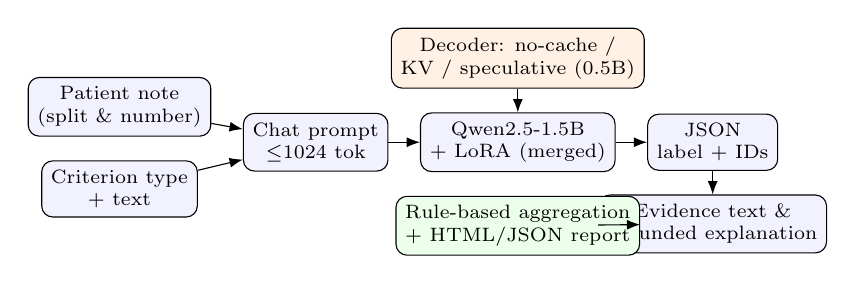
\begin{tikzpicture}[node distance=3mm and 4mm, every node/.style={font=\scriptsize},
 box/.style={draw,rounded corners,align=center,minimum height=6mm,fill=blue!5}]
\node[box] (note) {Patient note\\(split \& number)};
\node[box,below=of note] (crit) {Criterion type\\+ text};
\node[box,right=of note,yshift=-4.5mm] (prompt) {Chat prompt\\$\le$1024 tok};
\node[box,right=of prompt] (lm) {Qwen2.5-1.5B\\+ LoRA (merged)};
\node[box,above=of lm,fill=orange!10] (dec) {Decoder: no-cache /\\KV / speculative (0.5B)};
\node[box,right=of lm] (json) {JSON\\label + IDs};
\node[box,below=of json] (exp) {Evidence text \&\\grounded explanation};
\node[box,below=of lm,fill=green!8] (agg) {Rule-based aggregation\\+ HTML/JSON report};
\draw[-Latex] (note) -- (prompt); \draw[-Latex] (crit) -- (prompt); \draw[-Latex] (prompt) -- (lm);
\draw[-Latex] (dec) -- (lm); \draw[-Latex] (lm) -- (json); \draw[-Latex] (json) -- (exp); \draw[-Latex] (exp) -- (agg);
\end{tikzpicture}
\caption{System architecture and application workflow.}\label{fig:arch}\end{figure}

\subsection{KV-Cached Autoregressive Decoding}
Both decoders call the model's forward pass directly; \texttt{generate()} is never used.
The \emph{reference} path re-encodes the full sequence at every step (\texttt{use\_cache=False}).
The \emph{cached} path runs one prefill over the $P$ prompt tokens, which stores per-layer tensors
$K,V\in\mathbb{R}^{1\times2\times P\times128}$ in a \texttt{DynamicCache}. Each decode step then feeds only
the newest token.
(i) \emph{Positions:} \texttt{position\_ids = cache\_position = [past\_len]}, so RoPE rotates the
new query and key at their true absolute position. Reusing position 0 would silently corrupt the
relative-position structure.
(ii) \emph{Masking:} the 2-D attention mask has length past\_len+1, all ones. A single new query may
attend to every cached key, which is exactly the causal constraint for the last row. During multi-token
speculative verification, the model's 4-D mask keeps the new block causal while exposing the full cache.
(iii) \emph{Cache growth:} the code asserts that the cache grows by exactly one position per step.
Its size is $2LH_{kv}d\cdot T\cdot2$ bytes.
(iv) \emph{Numerics:} fp16 matrix products with different shapes (full-sequence vs.\ one-row) may
round differently. A greedy flip can occur only when the top-2 logit margin is tiny, so the benchmark
records the margin at any first mismatch.

\subsection{Tiled Attention with Online Softmax}
The reference computes $\mathrm{softmax}(QK^\top/\sqrt d+M)V$ in fp32 with row-max subtraction and
handles fully masked rows. The tiled variant (Alg.~\ref{alg:tiled}) loops over query blocks and key
blocks. It keeps the running maximum $m$, normalizer $\ell$ and unnormalized accumulator, and never
forms the $L\times L$ matrix. Fully masked key blocks above the diagonal are skipped. Only blocks that
cross the diagonal are masked. Causal masks are bottom-right aligned, so the same code covers prefill
($L_q=L_k$), single-token decode ($L_q=1$) and speculative verification blocks.

\begin{algorithm}[t]\caption{Tiled causal attention with online softmax}\label{alg:tiled}
\begin{algorithmic}[1]\scriptsize
\For{each query block $Q_i$}
 \State $m\gets-\infty$, $\ell\gets0$, $A\gets0$
 \For{each key block $j$ not entirely in the causal future of $Q_i$}
  \State $S\gets Q_iK_j^\top/\sqrt d$; mask $S$ if block crosses the diagonal
  \State $m'\gets\max(m,\mathrm{rowmax}(S))$; $P\gets e^{S-m'}$; $\alpha\gets e^{m-m'}$
  \State $\ell\gets\alpha\ell+\mathrm{rowsum}(P)$; $A\gets\alpha A+PV_j$; $m\gets m'$
 \EndFor
 \State $O_i\gets A/\ell$
\EndFor
\end{algorithmic}\end{algorithm}

\subsection{Greedy Speculative Decoding}\label{sec:specmethod}
Target and draft share the Qwen2.5 tokenizer, so token IDs are directly comparable. Each iteration
proceeds as follows. (1) The draft proposes $k$ tokens greedily after the last target-verified token $x$.
(2) The target scores $[x,d_1..d_k]$ in \emph{one} forward pass, giving greedy predictions $g_0..g_k$.
(3) The longest prefix with $d_i=g_{i-1}$ is accepted. (4) $g_a$ is appended as the correction token
(on rejection) or bonus token (on full acceptance), so each target pass commits $a+1$ tokens.
(5) Both caches are \emph{cropped} back to the committed length, discarding the K/V of rejected
drafts. Draft tokens committed but not yet seen by the draft cache are kept pending and fed at the next
round. Greedy acceptance makes the output provably identical to target greedy decoding, which we verify
token by token.

\subsection{Browser Application}
A Gradio application (\texttt{start\_app.bat} / \texttt{app.py}, \url{http://127.0.0.1:7860}) accepts an unseen
free-text note, which is sentence-split and numbered. It also accepts inclusion and exclusion criteria,
one per line, and a decoding mode. The app validates inputs (empty or short note, missing or too many
criteria, out-of-memory, unparseable output) without crashing. For each criterion it shows the label,
cited IDs, verbatim evidence, explanation, raw output and latency. It lists criteria that need more
information and gives an \emph{explicitly rule-based} preliminary outcome. Any failed inclusion or
triggered exclusion means \emph{likely ineligible}. Otherwise any \emph{not enough information} means
\emph{undetermined}. Otherwise the outcome is \emph{potentially eligible}. This is an aggregation, not a
ground-truth label. HTML and JSON reports carry provenance: model, adapter, decoding settings, a note hash
and a timestamp. Live tabs run the three decoders and the three attention implementations on the user's
input. A banner states that the system is an educational prototype, not an enrollment decision tool.

\section{Experimental Setup and Metrics}
All decoding is deterministic greedy with \texttt{max\_new\_tokens}=48, stopping at
\texttt{<|im\_end|>}, in fp16, using the KV-cached decoder. The zero-shot and fine-tuned models receive
\emph{identical} prompts. Outputs are parsed as JSON. An invalid label defaults to
\emph{not enough information} and is counted as a parse error, never silently mapped to a decisive label.
\textbf{Classification:} accuracy, macro-F1, per-class P/R/F1 and confusion matrices, overall and per
criterion type. \textbf{Evidence:} micro P/R/F1 pools (record, sentence) pairs over all records, so
citations on empty-gold records count as false positives. Macro P/R/F1 averages over records with
non-empty gold evidence, and an empty prediction scores 0 there. The fraction of empty-gold records with
an empty prediction is reported separately. \textbf{Benchmarks:} one warm-up run, then repeated runs timed
with \texttt{time.perf\_counter} after \texttt{torch.cuda.synchronize}. Medians are reported, and peak
memory comes from \texttt{torch.cuda.max\_memory\_allocated}.

\section{Results and Discussion}
\subsection{Fine-Tuning and Before/After Comparison}
Fig.~\ref{fig:curve} shows the training and validation loss. Table~\ref{tab:ba} and Fig.~\ref{fig:ba} compare
the zero-shot and LoRA models on identical validation and test examples.
The zero-shot model reaches only 0.170 test accuracy (macro-F1 0.158). It answers \emph{not applicable}
for most exclusion criteria (exclusion accuracy 0.061) and cites nearly every sentence. Training took 74
optimizer steps (6.7\,min on a T4, peak 11.1\,GB). Validation loss fell from 0.149 to 0.131 at step 60,
the selected checkpoint, while training loss kept dropping to about 0.10. That gap signals the onset of
overfitting on only 602 examples. After LoRA, test accuracy rises to 0.704 and macro-F1 to 0.434, and
validation shows the same picture (0.709 / 0.342). Neither model produced a single parse error, so the
JSON schema in the prompt was enough to fix the output \emph{format}. Fine-tuning changed the
\emph{decisions}.

\begin{figure}[t]\centering\fig{training_curve_adapter.png}{\columnwidth}
\caption{LoRA training and validation loss (answer tokens only).}\label{fig:curve}\end{figure}

\begin{table*}[t]\centering\caption{Criterion-level label metrics before (zero-shot) and after LoRA fine-tuning; greedy, identical prompts.}\label{tab:ba}
\begin{tabular}{llccccccc}\toprule
Split & Model & Acc. & Macro-F1 & Incl. Acc. & Incl. M-F1 & Excl. Acc. & Excl. M-F1 & Parse err.\\\midrule
\tbl{before_after.tex}
\bottomrule\end{tabular}\end{table*}

\begin{figure}[t]\centering\fig{before_after.png}{\columnwidth}
\caption{Before vs.\ after fine-tuning (accuracy, macro-F1, evidence micro-F1).}\label{fig:ba}\end{figure}

\subsection{Detailed Classification Metrics (held-out test)}
Table~\ref{tab:perclass} gives per-class metrics and Fig.~\ref{fig:cm} the confusion matrices of the
fine-tuned model on the test split.
The gap between accuracy and macro-F1 reveals \textbf{majority-class collapse}. For exclusion
criteria the model predicts \emph{not excluded} for all 131 test records (recall 1.00, precision 0.69).
\emph{Not enough information} and \emph{not applicable} are never predicted for exclusions. For inclusion
criteria, \emph{included} has precision 1.00 but recall 0.59, and \emph{not enough information} (recall
1.00) absorbs every \emph{not included} and \emph{not applicable} case. Always answering the majority label
per criterion type would give 0.626 test accuracy, so the fine-tuned model beats this baseline only through
the inclusion criteria. The cause is the extreme imbalance of the training split (292 \emph{not excluded}
vs.\ 8 \emph{excluded}, 5 inclusion \emph{not applicable}) under an unweighted cross-entropy objective.
Class-weighted loss or oversampling of minority labels is the most direct remedy (Section~VII).

\begin{table}[t]\centering\caption{Per-class test metrics (fine-tuned).}\label{tab:perclass}
\resizebox{\columnwidth}{!}{\begin{tabular}{llcccc}\toprule
Type & Class & P & R & F1 & Support\\\midrule
\tbl{per_class_test.tex}
\bottomrule\end{tabular}}\end{table}

\begin{figure*}[t]\centering
\fig{confusion_test_base.png}{0.48\textwidth}\hfill\fig{confusion_test_finetuned.png}{0.48\textwidth}
\caption{Test confusion matrices, zero-shot (left) and fine-tuned (right). NEI = not enough information.}\label{fig:cm}\end{figure*}

\subsection{Evidence Sentence Localization}
Table~\ref{tab:evid} reports evidence retrieval metrics.
Evidence localization improves the most. Test micro-F1 rises from 0.183 to 0.545 and macro-F1 over
records with gold evidence from 0.297 to 0.576. The gain comes from \emph{precision} (0.106$\rightarrow$0.519)
at similar recall (0.670$\rightarrow$0.574). The base model cites indiscriminately, while the adapted model
cites selectively and leaves the list empty for 87.6\% of records whose gold evidence is empty (base: 44.8\%).
Because every cited ID indexes an original note sentence, each prediction in the application links back to
verbatim evidence.

\begin{table*}[t]\centering\caption{Evidence-sentence retrieval. Macro averages over records with non-empty gold; ``empty agr.'' = share of empty-gold records with no citation.}\label{tab:evid}
\begin{tabular}{llccccccc}\toprule
Split & Model & Micro P & Micro R & Micro F1 & Macro P & Macro R & Macro F1 & Empty agr.\\\midrule
\tbl{evidence.tex}
\bottomrule\end{tabular}\end{table*}

\subsection{Error Analysis}
Table~\ref{tab:errors} lists representative test errors, sampled per category. The full cases with
evidence text are in \texttt{results/error\_analysis.md}.
On the 206 test records the error categories are: \emph{unsupported} decisive label where the gold is
\emph{not enough information} (28), \emph{missed information} (18), confusions involving \emph{not applicable}
(15), and correct label with disjoint evidence (14). There were no direct contradictions (e.g.\ included
$\leftrightarrow$ not included) and no parse errors. E1--E2 are the most important failure. Criteria the note
never mentions (pre-operative GFR, previous axillary surgery) are labelled \emph{not excluded} with
\emph{no cited sentence}. This treats absence of evidence as proof, which is exactly the behaviour the task
warns against, and it inflates a ``potentially eligible'' aggregate. The application therefore marks every
decisive label without a citation as weakly supported. E3--E4 are the opposite case: the expert inferred
\emph{not included} (the patient underwent catheterization, not endarterectomy) without citing a sentence,
and the model abstained. E5--E6 show that \emph{not applicable} vs.\ \emph{not excluded}/\emph{not enough
information} is partly a matter of annotator convention (pregnancy for a 67-year-old woman; birth control for
a sexually inactive adolescent), so some of these ``errors'' are label ambiguity. E7--E8 have the right label
but omit the age sentence the expert cited, which shows that evidence recall suffers on ``obviously
satisfied'' criteria.

\begin{table*}[t]\centering\caption{Representative test-set errors of the fine-tuned model.}\label{tab:errors}
\resizebox{\textwidth}{!}{\begin{tabular}{llllll}\toprule
ID & Category & Type & Criterion & Gold & Predicted\\\midrule
\tbl{errors.tex}
\bottomrule\end{tabular}}\end{table*}

\subsection{KV-Cached Decoding}
Table~\ref{tab:kv} and Fig.~\ref{fig:kv} compare the cached and reference decoders.
The cached decoder reproduces the reference tokens exactly in all three settings (370/32, 517/64,
1043/128 input/output tokens). That holds even though the smallest top-2 logit margin seen was 0.031, close to
fp16 resolution, so no mismatch needed investigating. Prefill costs are equal (one forward pass over the prompt,
59--213\,ms). The decode phase differs sharply. With the cache, throughput stays flat at about 30\,tok/s regardless
of context length. Without it, throughput falls from 14.2 to 8.9 to 4.1\,tok/s because every step re-encodes the
whole sequence ($O(T^2)$ total work). End-to-end speed-ups are 2.0$\times$, 3.3$\times$ and 7.0$\times$ and
grow with length. Peak memory is dominated by the 3.07\,GB of fp16 weights. The cache itself is only
11--32\,MB, matching the analytic 28\,KB/token of GQA with 2 KV heads, so the memory curves of the two paths
nearly coincide (Fig.~\ref{fig:kv}). Even cached decoding (33\,ms/token) is well above the bandwidth bound
(3.1\,GB / 320\,GB/s $\approx$ 10\,ms). At batch size 1, per-layer kernel-launch and Python overhead dominate.

\begin{table}[t]\centering\caption{KV cache vs.\ no-cache greedy decoding (fine-tuned target, T4, fp16, median of 3).}\label{tab:kv}
\resizebox{\columnwidth}{!}{\begin{tabular}{llccccc}\toprule
In/Out & Mode & Prefill ms & Decode s & Decode tok/s & Peak MB & Equal\\\midrule
\tbl{kv.tex}
\bottomrule\end{tabular}}\end{table}

\begin{figure}[t]\centering\fig{kv_bench.png}{\columnwidth}
\caption{Latency and peak memory, KV cache vs.\ no cache.}\label{fig:kv}\end{figure}

\subsection{Tiled Attention}
Table~\ref{tab:attn} validates the tiled kernel and Table~\ref{tab:attnperf} / Fig.~\ref{fig:attn} compare cost.
All eight cases pass, including non-multiple-of-block lengths, a non-causal case, single-token decode
($L_q{=}1$) and a 5-token speculative verification block with bottom-right causal alignment. The maximum
error is $3.6\times10^{-7}$ in fp32 and $9.7\times10^{-4}$ in fp16. The latter equals the error of PyTorch's
fused SDPA against the same fp32 reference ($9.9\times10^{-4}$), i.e.\ fp16 rounding. In memory the tiled kernel
behaves as theory predicts. The reference's peak grows quadratically (33\,MB$\rightarrow$2.38\,GB from $L$=256 to
4096) because it materializes the $L\times L$ score matrix. The tiled version grows linearly (25$\rightarrow$48\,MB),
close to the fused kernel (44\,MB). In time it is 3.7--4.6$\times$ \emph{slower} than the reference and up to
160$\times$ slower than fused SDPA. The reasons: it issues hundreds of small matmul, exp and max kernels from a
Python loop; every tile round-trips through GPU global memory instead of staying in on-chip SRAM/registers; and
nothing is fused. FlashAttention~\cite{dao2022flashattention} performs the same recurrence inside one fused
kernel, which is why its speed and memory benefits coincide.

\begin{table}[t]\centering\caption{Tiled vs.\ reference attention error (C=causal, F=full; reference in fp32).}\label{tab:attn}
\resizebox{\columnwidth}{!}{\begin{tabular}{lcccccc}\toprule
B$\times$H$\times L_q\times L_k\times$D & Mask & dtype & Block & Max err & Mean err & Result\\\midrule
\tbl{attn_correct.tex}
\bottomrule\end{tabular}}\end{table}

\begin{table}[t]\centering\caption{Causal attention runtime (ms) and peak memory (MB), 12 heads, $d$=64, fp16.}\label{tab:attnperf}
\resizebox{\columnwidth}{!}{\begin{tabular}{lcccccc}\toprule
$L$ & Ref ms & Ref MB & Tiled ms & Tiled MB & SDPA ms & SDPA MB\\\midrule
\tbl{attn_perf.tex}
\bottomrule\end{tabular}}\end{table}

\begin{figure}[t]\centering\fig{attention_bench.png}{0.85\columnwidth}
\caption{Attention runtime vs.\ sequence length.}\label{fig:attn}\end{figure}

\subsection{Speculative Decoding}\label{sec:spec}
Table~\ref{tab:spec} and Fig.~\ref{fig:spec} report token equality, acceptance and speed.
All 6 configurations produce output token-identical to greedy target decoding on all 12 prompts,
including iterations with rejections. This confirms the accept/correct logic and the cache rollback.
Fine-tuning the draft on the same data raises acceptance from 0.73/0.67/0.61 to 0.90/0.86/0.83 for
$k$=2/4/6, and up to 4.9 tokens are accepted per target pass. Yet every configuration is \emph{slower} than
plain greedy decoding (0.74--0.94$\times$). The best case is the fine-tuned draft with $k$=2 at 25.9 vs.\
27.6\,tok/s. The timing breakdown explains why. For the fine-tuned draft at $k$=4, drafting takes 4.3\,s
against 1.5\,s of verification. Under the model of~\cite{leviathan2023fast}, the expected tokens per iteration
$(1-\alpha^{k+1})/(1-\alpha)$ must exceed the relative iteration cost $ck+1$, where $c$ is the draft-to-target
per-token cost ratio. With $\alpha$=0.86 and $k$=4 this needs $c<0.70$. At batch size 1 on a T4, though, both
models are dominated by per-layer launch overhead, and the 24-layer draft is nearly as slow per token as the
28-layer target ($c\approx0.7$--$0.8$). The JSON answers are also short (about 15 tokens), so the second prefill
and per-iteration bookkeeping weigh heavily. A speed-up would need a much cheaper draft (a few layers, or
prompt-lookup $n$-grams) or a larger, memory-bound target such as a 7B model, where $c$ falls to about 0.1.
The draft adds about 1\,GB of weights, and the cache overhead is negligible.

\begin{table*}[t]\centering\caption{Greedy speculative decoding vs.\ greedy target decoding (same prompts; draft Qwen2.5-0.5B-Instruct, base or LoRA-tuned).}\label{tab:spec}
\begin{tabular}{lcccccccc}\toprule
Decoder & $k$ & Accept. rate & Accepted/iter & Total s & Tok/s & Speed-up & Peak MB & Token-equal\\\midrule
\tbl{spec.tex}
\bottomrule\end{tabular}\end{table*}

\begin{figure}[t]\centering\fig{spec_bench.png}{0.85\columnwidth}
\caption{Speculative speed-up vs.\ draft length.}\label{fig:spec}\end{figure}

\subsection{Application}
Fig.~\ref{fig:app} shows the screening and benchmark views on an unseen validation patient.
\begin{figure}[t]\centering\fig{screenshot_screening.png}{\columnwidth}\\[1mm]\fig{screenshot_benchmark.png}{\columnwidth}
\caption{Browser application: criterion-level screening with evidence (top) and live decoding benchmark (bottom).}\label{fig:app}\end{figure}

\subsection{Design Decisions, Alternatives and Difficulties}
\emph{Alternatives considered:} full fine-tuning (rejected: optimizer memory), QLoRA (not needed at 1.5B;
quantization would also perturb the speculative equality test), a classification head (rejected: it
cannot emit evidence IDs and would not exercise autoregressive decoding), and label-before-evidence
ordering (rejected: the label should be conditioned on the cited evidence).
\emph{Difficulties:} the first training run (fp32 frozen base, batch 4) ran out of memory on the 16\,GB T4.
The logits tensor $4\times649\times151{,}936$ alone needs about 1.6\,GB, and each step took 21\,s. The final
configuration stores the frozen base in fp16 (the T4 has no native bf16), up-casts only the LoRA matrices to
fp32 for fp16 mixed precision, and uses batch 2 with 8 accumulation steps (peak 11.1\,GB). The
4\,GB local GPU cannot hold target and draft together in fp16, so the application places the draft on the
CPU when memory is short, which makes local speculation slower than on the T4. One dataset row has a null
criterion. A newer \texttt{transformers} release changed the cache internals, so versions are pinned.

\section{Limitations}
The test set has only 8 patients (206 criteria) and no \emph{excluded} example, so the metrics have
high variance and some per-class scores are undefined. The adapted model collapses to majority labels for
exclusion criteria and sometimes treats unmentioned conditions as \emph{not excluded}. Class-weighted loss,
oversampling, and an explicit abstention rule for uncited decisive labels are the next steps. Hyperparameters
were not searched beyond validation-loss checkpoint selection because of the time budget. The SIGIR notes are short, synthetic-style
summaries; real EHR notes are longer and noisier, and the free-text sentence splitter is heuristic.
Explanations are templated from evidence rather than generated, which guarantees grounding but
limits their reasoning content. The educational tiled kernel runs in Python loops and is slower than
fused SDPA, and speculative gains depend on hardware and draft agreement. The system is a research
screening prototype and must not be used for enrollment decisions.

\section{Conclusion}
A 1.5B-parameter open model adapted with LoRA on 602 criterion annotations yields a structured,
evidence-citing criterion matcher that runs on a 4\,GB consumer GPU. It improves held-out accuracy from 0.17
to 0.70 and evidence F1 from 0.18 to 0.55, but its minority-class recall, especially for exclusion criteria,
remains the main weakness. The KV-cached, tiled-attention
and speculative decoders were implemented from first principles and validated for exact or
tolerance-level agreement with their references, and the measurements explain when each one helps.

\bibliographystyle{IEEEtran}
\begin{thebibliography}{99}
\bibitem{jin2024trialgpt} Q.~Jin, Z.~Wang, C.~S.~Floudas, F.~Chen, C.~Gong, D.~Bracken-Clarke, E.~Xue, Y.~Yang, J.~Sun, and Z.~Lu, ``Matching patients to clinical trials with large language models,'' \emph{Nature Communications}, vol.~15, art.~9074, 2024.
\bibitem{koopman2016test} B.~Koopman and G.~Zuccon, ``A test collection for matching patients to clinical trials,'' in \emph{Proc. ACM SIGIR}, 2016, pp.~669--672.
\bibitem{vaswani2017attention} A.~Vaswani \emph{et al.}, ``Attention is all you need,'' in \emph{Proc. NeurIPS}, 2017.
\bibitem{su2024roformer} J.~Su, M.~Ahmed, Y.~Lu, S.~Pan, W.~Bo, and Y.~Liu, ``RoFormer: Enhanced transformer with rotary position embedding,'' \emph{Neurocomputing}, vol.~568, 2024.
\bibitem{ainslie2023gqa} J.~Ainslie \emph{et al.}, ``GQA: Training generalized multi-query transformer models from multi-head checkpoints,'' in \emph{Proc. EMNLP}, 2023.
\bibitem{qwen2025} Qwen Team, ``Qwen2.5 technical report,'' arXiv:2412.15115, 2024.
\bibitem{grattafiori2024llama} A.~Grattafiori \emph{et al.}, ``The Llama 3 herd of models,'' arXiv:2407.21783, 2024.
\bibitem{hu2022lora} E.~J.~Hu \emph{et al.}, ``LoRA: Low-rank adaptation of large language models,'' in \emph{Proc. ICLR}, 2022.
\bibitem{dettmers2023qlora} T.~Dettmers, A.~Pagnoni, A.~Holtzman, and L.~Zettlemoyer, ``QLoRA: Efficient finetuning of quantized LLMs,'' in \emph{Proc. NeurIPS}, 2023.
\bibitem{pope2023efficiently} R.~Pope \emph{et al.}, ``Efficiently scaling transformer inference,'' in \emph{Proc. MLSys}, 2023.
\bibitem{kwon2023vllm} W.~Kwon \emph{et al.}, ``Efficient memory management for large language model serving with PagedAttention,'' in \emph{Proc. SOSP}, 2023.
\bibitem{milakov2018online} M.~Milakov and N.~Gimelshein, ``Online normalizer calculation for softmax,'' arXiv:1805.02867, 2018.
\bibitem{dao2022flashattention} T.~Dao, D.~Y.~Fu, S.~Ermon, A.~Rudra, and C.~R\'e, ``FlashAttention: Fast and memory-efficient exact attention with IO-awareness,'' in \emph{Proc. NeurIPS}, 2022.
\bibitem{leviathan2023fast} Y.~Leviathan, M.~Kalman, and Y.~Matias, ``Fast inference from transformers via speculative decoding,'' in \emph{Proc. ICML}, 2023.
\bibitem{chen2023accelerating} C.~Chen, S.~Borgeaud, G.~Irving, J.-B.~Lespiau, L.~Sifre, and J.~Jumper, ``Accelerating large language model decoding with speculative sampling,'' arXiv:2302.01318, 2023.
\end{thebibliography}

\appendix[AI-Use Statement]
An AI coding assistant (Claude, Anthropic) was used to draft code (data preparation, training,
decoders, application) and parts of this report. The author ran every script, checked the
correctness tests (token equality, attention error bounds), inspected the outputs and can explain
and modify every component. Libraries used: PyTorch, Hugging Face Transformers/PEFT, scikit-learn,
Gradio. TrialGPT code was consulted as a reference only and was not executed or copied.
\end{document}
